\begin{table}[tb]
\renewcommand{\arraystretch}{1}
    \centering
    \resizebox{\textwidth}{!}{
    \begin{tabular}{ccccccc}
    %\toprule
    \toprule
    \rowcolor{hdrcolor}
    \textbf{Field}  & \textbf{Spin} & \textbf{Channel} & \boldmath$[C_{\ell q}^{(1)}]_{3333}/\Lambda^2$ & \boldmath$[C_{\ell q}^{(3)}]_{3333}/\Lambda^2$ & \textbf{Unitarity Bound} & \textbf{Plot} \\
    \midrule
    % $\omega_1$ & $(3,1)_{-\displaystyle\frac{1}{3}}$ & $0$ & $s$ & $\displaystyle\frac{|[y^{q\ell}_{\omega_1}]_{33}|^2}{4M^2_{\omega_1}}$ & $\displaystyle\frac{-|[y^{q\ell}_{\omega_1}]_{33}|^2}{4M^2_{\omega_1}}$ & $\displaystyle\frac{|[y^{q\ell}_{\omega_1}]_{33}|^2 s}{4\pi M^2_{\omega_1}}\leq 1$ & \makecell[c]{\includegraphics[scale = 0.5]{images/omega1.pdf}} \\
    % $\zeta$ & $(3,3)_{-\displaystyle\frac{1}{3}}$ & $0$ & $s$ & $3|[y^{q\ell}_{\zeta}]_{33}|^2/(4M^2_{\zeta})$ & $|[y^{q\ell}_{\zeta}]_{33}|^2/(4M^2_{\zeta})$ & $|[y^{q\ell}_{\zeta}]_{33}|^2\,s\leq 4\pi M^2_{\zeta}$ & \makecell[c]{\includegraphics[scale = 0.5]{images/zeta.pdf}} \\
    % $\mathcal{U}_2$ & $(3,1)_{\displaystyle\frac{2}{3}}$ & $1$ & $s$ & $-|[g_{\mathcal U_2}^{\ell q}]_{33}|^2/(2M^2_{\mathcal U_2})$ & $-|[g_{\mathcal U_2}^{\ell q}]_{33}|^2/(2M^2_{\mathcal U_2})$ & $|[g_{\mathcal U_2}^{\ell q}]_{33}|^2\,s\leq 4\pi M^2_{\mathcal U_2}$ & \makecell[c]{\includegraphics[scale = 0.5]{images/U2.pdf}} \\
    % $\mathcal{X}$ & $(3,3)_{\displaystyle\frac{2}{3}}$ & $1$ & $s$ & $-3|[g_{\mathcal X}]_{33}|^2/(8M^2_{\mathcal X})$ & $|[g_{\mathcal X}]_{33}|^2/(8M^2_{\mathcal X})$ & $|[g_{\mathcal X}]_{33}|^2\,s\leq \tfrac{16}{3}\pi M^2_{\mathcal X}$ & \makecell[c]{\includegraphics[scale = 0.5]{images/X.pdf}} \\
    % $\mathcal{B}$ & $(1,1)_{0}$ & $1$ & $t$ & $-[g_{\mathcal B}^\ell]_{33}[g_{\mathcal B}^q]_{33}/M^2_{\mathcal B}$ & $0$ & $|[g_{\mathcal B}^\ell]_{33}[g_{\mathcal B}^q]_{33}|\,s\leq 2\sqrt{3}\,\pi M^2_{\mathcal B}$ & \makecell[c]{\includegraphics[scale = 0.5]{images/B.pdf}} \\
    % $\mathcal{W}$ & $(1,3)_{0}$ & $1$ & $t$ & $0$ & $-[g_{\mathcal W}^\ell]_{33}[g_{\mathcal W}^q]_{33}/(4M^2_{\mathcal W})$ & $|[g_{\mathcal W}^\ell]_{33}[g_{\mathcal W}^q]_{33}|\,s\leq \tfrac{16}{3}\pi M^2_{\mathcal W}$ & \makecell[c]{\includegraphics[scale = 0.5]{images/W.pdf}} \\
    % \bottomrule
    $\omega_1\sim(3,1)_{-\frac{1}{3}}$ & $0$ & $s$ & $\displaystyle\frac{|[y^{q\ell}_{\omega_1}]_{33}|^2}{4M^2_{\omega_1}}$ & $\displaystyle\frac{-|[y^{q\ell}_{\omega_1}]_{33}|^2}{4M^2_{\omega_1}}$ & $\displaystyle\frac{|[y^{q\ell}_{\omega_1}]_{33}|^2 s}{4\pi M^2_{\omega_1}}\leq 1$ & \makecell[c]{\includegraphics[scale = 0.8,page=6]{images/UVfield.pdf}} \\
$\zeta\sim(3,3)_{-\frac{1}{3}}$ & $0$ & $s$ & $\displaystyle\frac{3|[y^{q\ell}_{\zeta}]_{33}|^2}{4M^2_{\zeta}}$ & $\displaystyle\frac{|[y^{q\ell}_{\zeta}]_{33}|^2}{4M^2_{\zeta}}$ & $\displaystyle\frac{|[y^{q\ell}_{\zeta}]_{33}|^2s}{4\pi M^2_{\zeta}}\leq 1$ & \makecell[c]{\includegraphics[scale = 0.8,page=5]{images/UVfield.pdf}} \\
$\mathcal{U}_2\sim(3,1)_{\frac{2}{3}}$ & $1$ & $s$ & $\displaystyle\frac{-|[g_{\mathcal U_2}^{\ell q}]_{33}|^2}{2M^2_{\mathcal U_2}}$ & $\displaystyle\frac{-|[g_{\mathcal U_2}^{\ell q}]_{33}|^2}{2M^2_{\mathcal U_2}}$ & $\displaystyle\frac{|[g_{\mathcal U_2}^{\ell q}]_{33}|^2s}{4\pi M^2_{\mathcal U_2}}\leq 1$ & \makecell[c]{\includegraphics[scale = 0.8,page=4]{images/UVfield.pdf}} \\
$\mathcal{X}\sim(3,3)_{\frac{2}{3}}$ & $1$ & $s$ & $\displaystyle\frac{-3|[g_{\mathcal X}]_{33}|^2}{8M^2_{\mathcal X}}$ & $\displaystyle\frac{|[g_{\mathcal X}]_{33}|^2}{8M^2_{\mathcal X}}$ & $\displaystyle\frac{3|[g_{\mathcal X}]_{33}|^2s}{16\pi M^2_{\mathcal X}}\leq 1$ & \makecell[c]{\includegraphics[scale = 0.8,page=3]{images/UVfield.pdf}} \\
$\mathcal{B}\sim(1,1)_{0}$ & $1$ & $t$ & $\displaystyle\frac{-[g_{\mathcal B}^\ell]_{33}[g_{\mathcal B}^q]_{33}}{M^2_{\mathcal B}}$ & $0$ & $\displaystyle\frac{|[g_{\mathcal B}^\ell]_{33}[g_{\mathcal B}^q]_{33}|s}{2\sqrt{3}\pi M^2_{\mathcal B}}\leq 1$ & \makecell[c]{\includegraphics[scale = 0.8,page=2]{images/UVfield.pdf}} \\
$\mathcal{W}\sim(1,3)_{0}$ & $1$ & $t$ & $0$ & $\displaystyle\frac{-[g_{\mathcal W}^\ell]_{33}[g_{\mathcal W}^q]_{33}}{4M^2_{\mathcal W}}$ & $\displaystyle\frac{3|[g_{\mathcal W}^\ell]_{33}[g_{\mathcal W}^q]_{33}|s}{16\pi M^2_{\mathcal W}}\leq 1$ & \makecell[c]{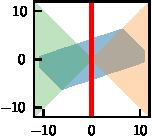
\includegraphics[scale = 0.8,page=1]{images/UVfield.pdf}} \\
\bottomrule
    \end{tabular}
    }
    \caption{Tree-level matching of single-field UV completions \cite{deBlas:2017xtg}
    onto $[O_{\ell q}^{(1)}]_{3333}$ and $[O_{\ell q}^{(3)}]_{3333}$. The penultimate
    column reports the associated perturbative unitarity bound, obtained as the most
    stringent of the constraints for $[C_{\ell q}^{(1)}]_{3333}$ and $[C_{\ell q}^{(3)}]_{3333}$ evaluated on the
    matched Wilson coefficients. The last column contains the plots in the plane $(s[C_{\ell q}^{(1)}]_{3333}/\Lambda^2, s[C_{\ell q}^{(3)}]_{3333}/\Lambda^2)$, where the blue, orange, and green regions correspond to those consistent with unitarity bounds and spin-$0$ and spin-$1$ sum-rule constraints, respectively, while the red lines indicate where each model lies: the scalar and vector leptoquarks are correctly classified by
    their spin, whereas the $t$-channel vectors evade the classification.}
    \label{tab:models}
\end{table}